\documentclass[12pt, a4paper]{article}

% Podpora cz
\usepackage[utf8]{inputenc}
\usepackage[IL2]{fontenc}
\usepackage[czech]{babel}
\usepackage{parskip}
\usepackage{graphicx}
%\usepackage[left=10cm,showframe]{geometry}

\title{Název článku}
\author{Adam Míka}

\begin{document}
\maketitle

Hello world!

\tableofcontents

Příliš žluťoučký kůň úpěl ďábelskými ody
Příliš žluťoučký kůň úpěl ďábel- \ skými ody
Příliš žluťoučký kůň úpěl ďábelskými ody
Příliš žluťoučký kůň úpěl ďábelskými ody
Příliš žluťoučký kůň úpěl ďábelskými ody

%\setcounter{section}{5}
\section{Předmluva}
Zatímco ve zbytku světa slyšíme stále častěji a hlasitěji, že klimatická
spravedlnost nesmí být založena jen na politikách určovaných bílými he-
terosexuálními muži, často ve středním věku a ze severní polokoule, Česku
a dalším zemím jako by se tento argument stále obloukem vyhýbal. Pří-
činou toho samozřejmě může být specifická historická zkušenost i to, že
zastoupení žen v rozhodovacích a vedoucích pozicích je stále velkou vý-
zvou pro celou českou společnost. Roli hraje možná i skutečnost, že čes-
ké klimatické hnutí specifickou situaci různých skupin obyvatelstva příliš
nereflektovalo – ani komunikačně, ani ve vnitřních strategiích. Velkou re-
volucí z hlediska větší senzitivity k zastoupení různých společenských sku-
pin byly první studentské stávky, jejichž výsledky jsou neoddiskutovatelně
spojeny s tím, že je prosadily studentky a studenti středních škol. Vývoj re-
lativně mladého klimatické hnutí, které vyrostlo ze staršího environmen-
tálního hnutí, už stihla narušit pandemie covidu-19 a válka na Ukrajině.

Je velkou otázkou, zda feministické hodnoty (které chápeme jako kla-
doucí důraz na respekt k jiným skupinám lidí) vlastně do klimatického
hnutí protékají. Na českém poli působí velké, silné environmentální or-
ganizace s tradicí, nezřídka vedené ženami. A potom je tu celá řada hnutí
založených na dobrovolnické práci, ale i ta mají reálné výsledky a profesi-
onální vnitřní strukturu. V expertních a veřejně viditelných pozicích však
stále dominují muži, stále je téměř nemožné v některých tématech najít
expertku do debaty či autorku komentáře v médiích. \ref{fig:feminismus}

Kdo jiný by mohl do
veřejné debaty přinést specifický pohled žen na důsledky klimatické krize \pageref{tab:metodologie}

\begin{figure}
    \centering
    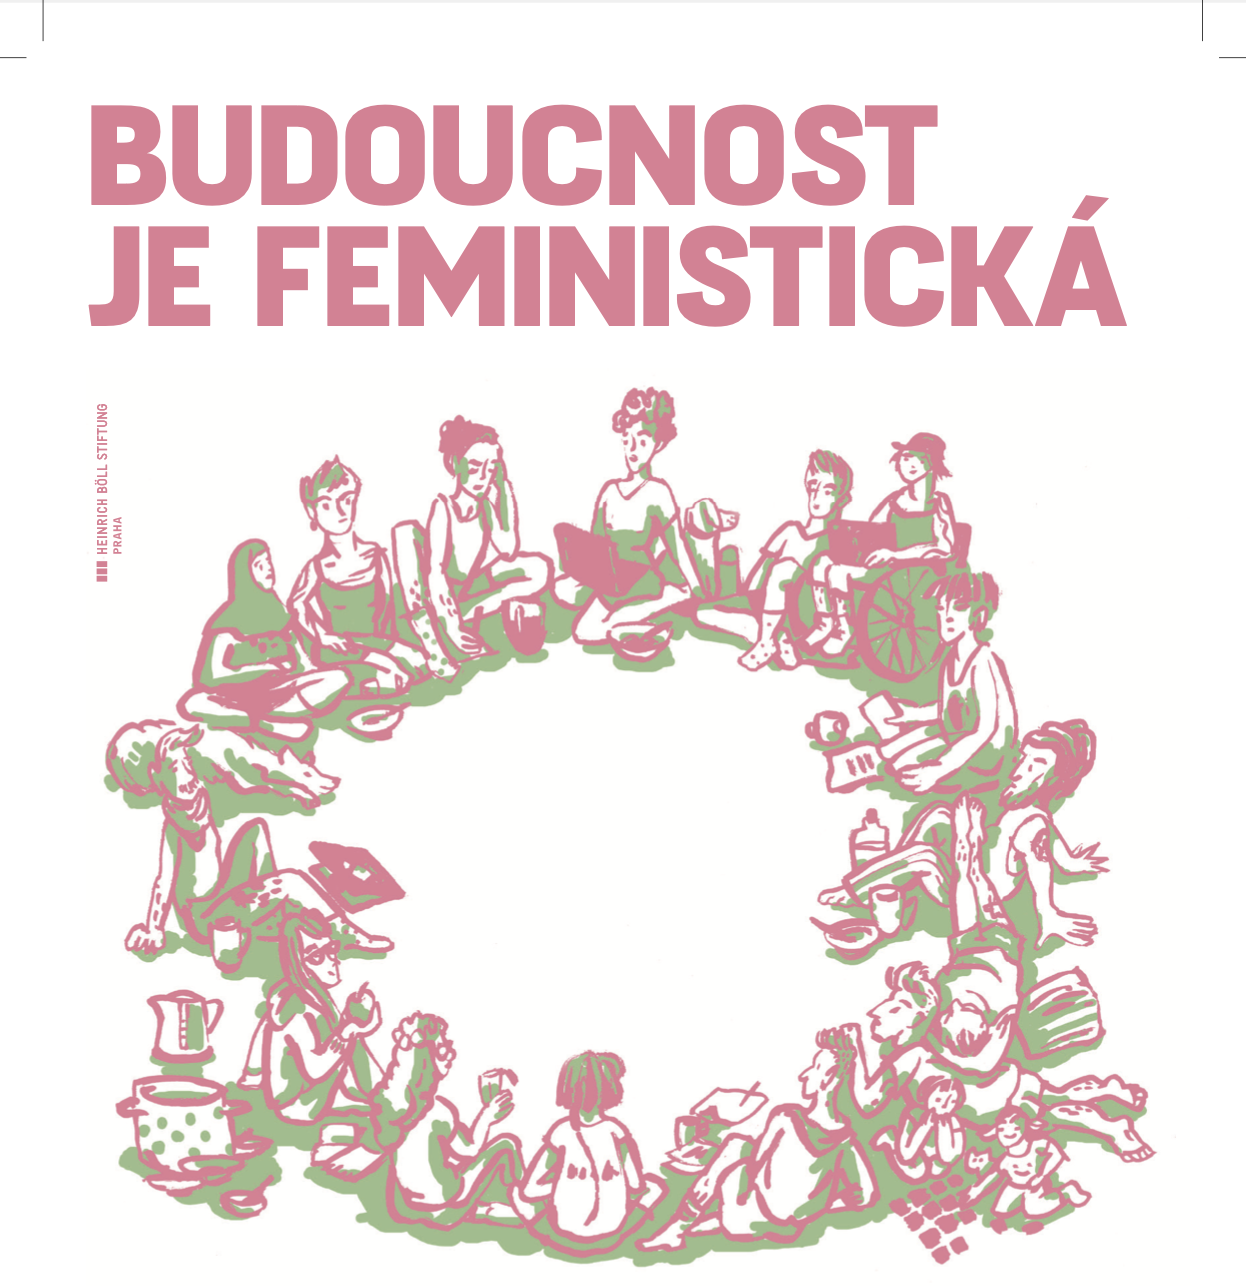
\includegraphics[width=.8\textwidth, angle=90]{img.png}
    \caption{Úsilí o genderovou rovnost je jedním z průřezových úkolů nadace
    Heinricha Bölla a odráží se v naší práci po celém světě.}
    \label{fig:feminismus}
\end{figure}

\begin{table}
\centering
\caption{Teoretická východiska, metodologie, pozicionalita}
\begin{tabular}{c|c}
    1 & 2 \\ \hline
    3 & 4
\end{tabular}
\label{tab:metodologie}
\end{table}

\begin{equation}
    % \iiint\limits_V x\,\mathrm{d}t
    \label{equ:rovnice}
\end{equation}

\section{Sekce s řezy písma}
\textit{Kurzíva}\\[2cm]
\textbf{tučně}
{\itshape\bfseries Kuzíva}

\begin{enumerate}
    \item prvni
    \item druhz
    \item Teoretická
    \item ctvrty
\end{enumerate}

\listoffigures

\end{document}